
Here we examine results of the simulations for a few setups

\begin{itemize}
  \item Fair coin
  \item Loaded coin
  \item Slightly loaded coin
\end{itemize}

\subsection{Fair coin}\label{sec:fair_coin}

Figure \ref{fig:iterations} presents the results of the cherry picked fair coin
experiment ($\theta_{\rm true}=0.5$). It was chosen to highlight potential stark
different outcomes of the three stop criterion algorithms. For comparison note that the posteriors
shown in Figure \ref{fig:posteriors} are three iterations of this figure.
(TB footnote: 1 - provide the sequence, 2 - reference to JK figure number)

As we can see from both figures at iteration 126 the credible interval (95\% HDI posterior) of HDI+ROPE is fully
outside of the ROPE making it confidently, though incorrectly, reject $\theta_{\rm null}$.
The Precision is the Goal stop criterion is met at iteration 598, where the credible
interval width
subpasses the precision goal of 0.08. Since the credible interval straddles the ROPE
the decision is inconclusive.
For the Enhanced Precision is the Goal the credible interval
meets both criterions at iteration 804: narrower than 0.08 precision goal and fully within the ROPE.
This results in correctly accepting $\theta_{\rm null}$.


\begin{figure}[h!]
  \centering
  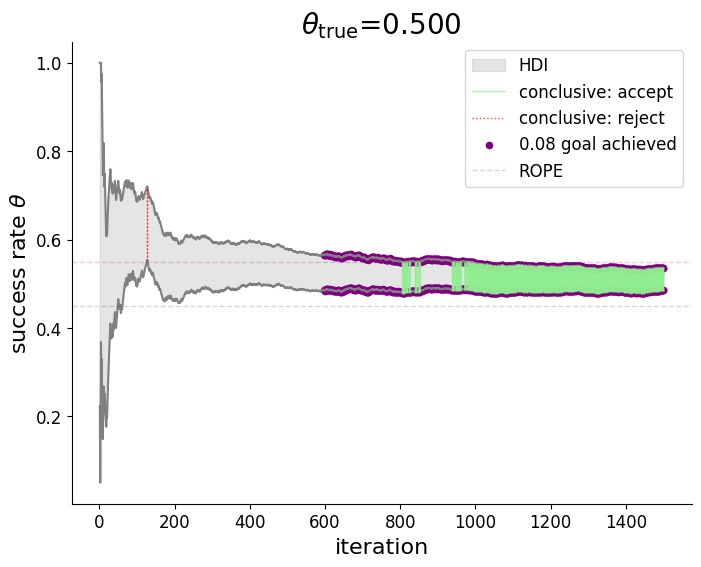
\includegraphics[width=1\textwidth]{cherry_iterations.png}
  \caption{Cherry picked fair coin sample demonstrating the varied outcomes by
  stop criterion mechanism. The vertical axis is the cumulative success rate
  at each iteration (horizontal axis).
  The gray band is the 95\% HDI of the posterior at each iteration.
  The highlighted iterations indicate where stop criterion trigger conditions are met:
  red dashed lines is when  $\theta_{\rm null}$ may be rejected, green solid lines
  is when he $\theta_{\rm null}$ may be accepted. Purple dots on the 95\% HDI boundaries
  indicated when the precision goal is achieved. Note that the posteriors of Figure \ref{fig:posteriors}
  are slices of this figure: HDI+ROPE is the the first red dashed line (iteration 126),
  Precision is the Goal is the first purple dot (598), and Enhanced Precision is the Goal is the second purple dot (598)
  is the first green line (804). The ROPE boundaries is represented by the dashed lines.
  }
  \label{fig:iterations}
\end{figure}

We continue to explore $M=500$ experiments and dispaly outcomes in
Figure \ref{fig:fair_iter_vs_rate} and summarise key stats in
Table \ref{tab:fair_iter_vs_rate}. 
(TK Ref JK figure number being additional information to his histograms).


\begin{figure}[h!]
  \centering
  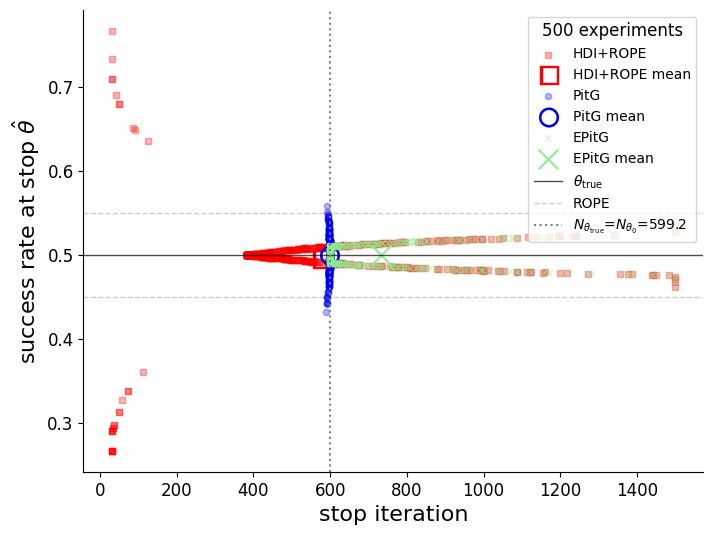
\includegraphics[width=1\textwidth]{fair_experiments_iter_vs_rate.png}
  \caption{Small symbols are individual experiment outcomes. Large are experiments
  mean values. When using HDI+ROPE as the stop criterion results in the red squares.
  Precision is the Goal as the criterion results in the blue circles
  and the Enhanced PitG as the green Xs. $\theta_{\rm true}$ is the solid line and
  the ROPE is the dashed lines. Summary stats are in Table \ref{tab:fair_iter_vs_rate}. TK: analytical results
  }
  \label{fig:fair_iter_vs_rate}
\end{figure}

In the Figure \ref{fig:fair_iter_vs_rate} the large symbols represent the 500 experiment outcome means 
(large red square, blue circle and X as per legend) show
that on average all methods yield, on average, unbiased outcomes, as per the
$\overline{\theta}$ column in Table \ref{tab:fair_iter_vs_rate}.


\begin{table}[h!]\label{tab:fair_iter_vs_rate}
  \begin{center}
  \begin{tabular}{c|c|c|c|c|c|c|c|c}
    \hline
    Algorithm & Accept & Reject & Conclusive & Inconclusive & $\overline{n}$ & $\sigma_n$ & $\overline{\theta}$ & $\sigma_{\hat{\theta}}$\\
    \hline
    HDI+ROPE & 0.928 & 0.06 & 0.988 & 0.012 & 576.6 & 281 & 0.4952 & 0.0502 \\
    PitG & 0.390 & 0.00 & 0.390 & 0.610 & 598.3 & 1.4 & 0.4994 & 0.01997 \\
    ePitG & 0.984 & 0.00 & 0.984 & 0.016 & 732.2 & 210 & 0.4998 & 0.0127\\
    \hline
  \end{tabular}
  \caption{Statistic summaries of 500 experiments of the three stop criteria shown in
  Figure \ref{fig:fair_iter_vs_rate}. {\it Accept}
  is the fraction of experiments which results in acceptence of $\theta_{\rm null}$,
  and similar in reverse for {\it Reject}. {\it Conclusive} is the sum of Accept
  and Reject and {\it Inconclusive} is its complementary.
  The mean stop iteration is $\overline{n}$ and the standard deviation $\sigma_n$
  The mean sample rate when the stop is triggered is $\overline{\theta}$ and its standard deviation is $\sigma_{\hat{\theta}}$.
  }
\end{center}
\end{table}

That said, HDI+ROPE falsely rejects $\theta_{\rm null}$ at a rate of 6\% 
whereas the precision methods do not have False Positives
(see Reject column in Table \ref{tab:fair_iter_vs_rate}).
(Note that if we relax the minimum sample size ($N_{\rm min}=0$) for the HDI+ROPE
algorithm the FPR increases to TK\%).
Precision is the Goal (blue circles) stops around iteration ~598 but decisions are 61\% inconclusive.
For conclusiveness of these 61\%, the Enhanced PitG (green Xs) requires more sampling 
resulting in only 1.6\% inconclusive outcomes by final iteration of $N_{\rm max}=1,500$.
This manifests in an average of $732.2\pm 210$ samples per experiment for the Enhanced PitG
compared to $598.3\pm 1.4$ for the Precision is the Goal.

Figure \ref{fig:fair_iter_vs_rate} highlights that after the "Precision stop barrier" at iteration 598 Enhanced Precision is the Goal and HDI+ROPE are the same algorithm.

In Figure \ref{fig:fair_decisions} we explore the decision rates of the three algorithms.
(TK reference to JK's graph).

\begin{figure}[h!]
  \centering
  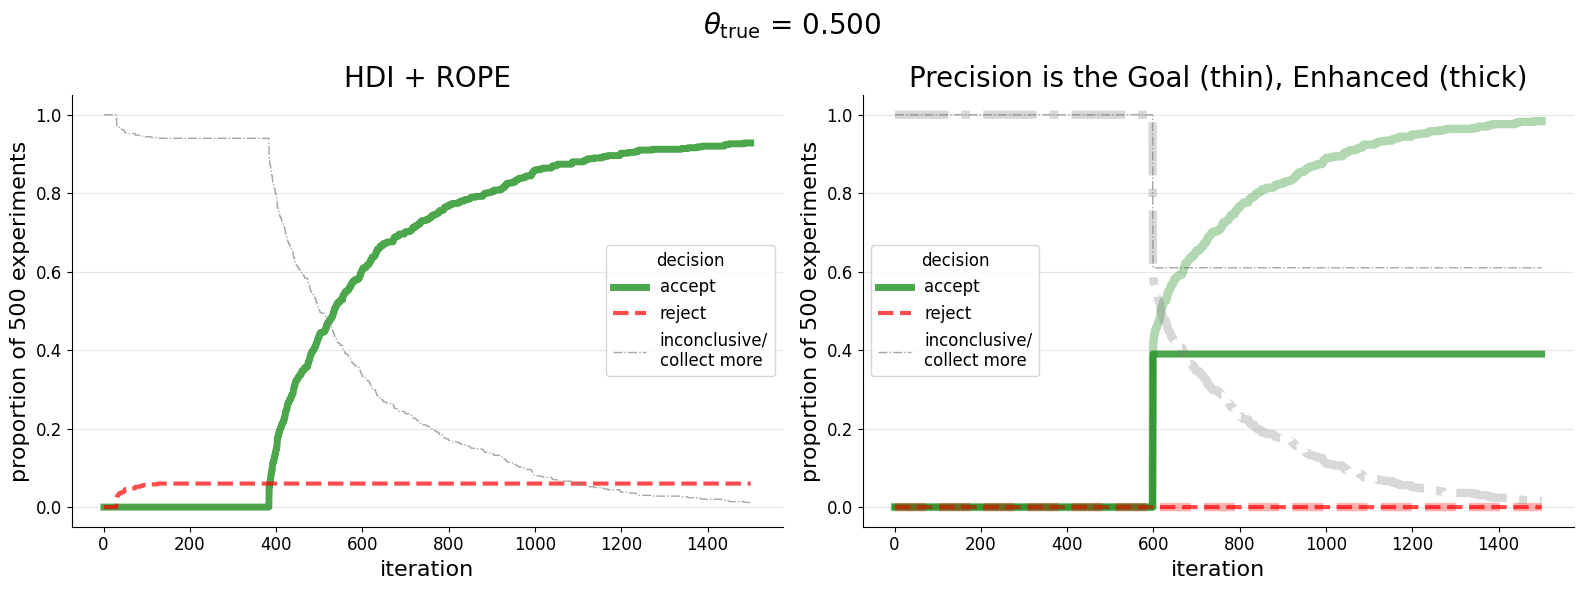
\includegraphics[width=1\textwidth]{fair_experiment_decision_rates.png}
  \caption{Similar information as in Figure \ref{fig:fair_iter_vs_rate} but focusing on
  the distribution of decisions. Left panel is for HDI+ROPE. Right panel are both
  precision based methods. Horizontal axis- iteration. Vertical axis- proportion of
  decisions made up to (and including) each iteration. The sum of Reject (red dashed),
  Accept (green solid) and Inconclusive/Collect-more- (gray dot-dashed) decisions at
  each iteration is 100\%.
  }
  \label{fig:fair_decisions}
\end{figure}

In the left panel of Figure \ref{fig:fair_decisions} we can see that for low $n$ the HDI+ROPE algorithm may result with rejection of
$\theta_{\rm null}$ ($6\%$ FPR) which the precision based methods do not (right panel).
At around iteration 400 (TK to be calculated) HDI+ROPE
gradually accepts $\theta_{\rm null}$. In Figure \ref{fig:fair_iter_vs_rate}
this manifests as the red squares being exactly on the $\theta_{\rm true}=0.5$ line
and then gradually moving towards the ROPE boundaries on both sides in a symmetric
manner due to the nature of the setup (e.g, we shall see that this symmetry
skewes as the coin becomes more loaded). The reason for this is that the mode of
the posteriors deviate slightly from the true value but the credible interval width
is narrow enough to be fully confined within the ROPE.

On the right panel of Figure \ref{fig:fair_decisions} and in Figure \ref{fig:fair_iter_vs_rate}
we see that Precision is the Goal triggers the stop criterion at iteration 598 for all of
it instances. This is by design - once the precision goal is met the algorithm stops.
For all instances we see this hapenning with very small variance of 1.4 iterations around 598.3.
As a result of this two step process we can clearly see that only 39\% of result in a decisive decision
(the decisive all correctly accept $\theta_{\rm null}$). 

The Enhanced Precision is the Goal (green Xs) is shown in these figure to be the natural extension
of the promise of the Precision is the Goal in terms of resulting in unbiassed outcomes. It's main 
benefit is that it is much more decisive. In the right panel of Figure \ref{fig:fair_decisions}
this manifests in the slow growing of the "accept" curve all the way to 98.4\% of the experiments
by the end of the $N_{\rm max}=1,500$ iterations.

As this binomial setup is well defined we see obvious trends
that may be described analytically. We discuss this more in detail
in Section TK but mention here that the expected stop iteration of Precision is the Goal
may be written as $$n = \frac{4 z_{*}^2}{\rm{CI}^2}p(1-p) - 1$$,
where 

\begin{itemize}
  \item $p$ is the success rate
  \item $CI$ is the precision goal of the credible interval. In our case 0.08.
  \item $z_{*}$ is the (TK). E.g, for 95\% quantile of the standard normal
  distribution $z_{*}=z_{0.05}=1.96$
\end{itemize}

For this fair coin instances we set $\theta_0=\theta_{\rm true}=\frac{1}{2}$ and obtain
$n=599.2$ as indicated as the dashed vertical line in Figure \ref{fig:fair_iter_vs_rate}.

We now turn to examining a loaded coins example where this is not the case.

\subsection{Loaded Coins}
We now examine cases where we should reject the null hypothesis of a fair conditions
$\theta_{0}=0.5$.

Results for these experiments are in Figures \ref{fig:loaded0pt6_iter_vs_rate} and
\ref{fig:loaded0pt6_decisions}, as well as Table \ref{tab:loaded0pt6_iter_vs_rate},
which are similar to those presented in the fair coin case in
Section \ref{sec:fair_coin}.

We see that for all three algorithms there is a 0\% FPR.
The HDI+ROPE algorithm, however, is highly biased with a mean
success rate at stop of 64.4\%. This can be explained by the all of experiments
which stopped fairly early. Both of the the precision based algorithms result in
unbiased outcomes.

We see that the Precision is the Goal algorithm, is still quite undecisive at a rate of 29.2\%
of experiments being inconclusive.

TODO: add calculation of the expected stop iteration for the Precision is the Goal algorithm for the 
inconclusive and conclusive

\subsubsection{$\theta_{\rm true}=0.6$}

\begin{figure}[h!]
  \centering
  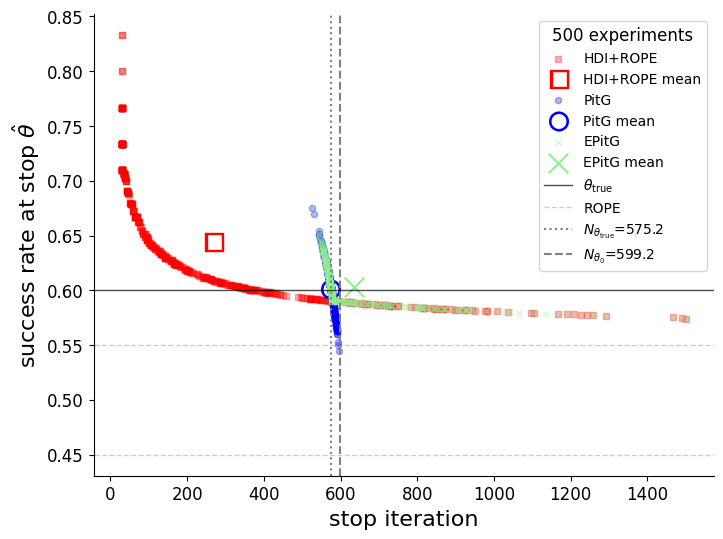
\includegraphics[width=1\textwidth]{loaded0pt6_experiments_iter_vs_rate.png}
  \caption{Similar to Figure \ref{fig:loaded_iter_vs_rate} but with
  loaded coin $\theta_{\rm true}=0.6$.
  Small symbols are individual experiment outcomes. Large are experiments
  mean values. When using HDI+ROPE as the stop criterion results in the red squares.
  Precision is the Goal as the criterion results in the blue circles
  and the Enhanced PitG as the green Xs. $\theta_{\rm true}$ is the solid line and
  the ROPE is the dashed lines. Summary stats are in Table \ref{tab:fair_iter_vs_rate}. TK: analytical results
  }
  \label{fig:loaded0pt6_iter_vs_rate}
\end{figure}


\begin{table}[h!]\label{tab:loaded0pt6_iter_vs_rate}
  \begin{center}
  \begin{tabular}{c|c|c|c|c|c|c|c|c}
    \hline
    Algorithm & Accept & Reject & Conclusive & Inconclusive & $\overline{n}$ & $\sigma_n$ & $\overline{\theta}$ & $\sigma_{\hat{\theta}}$\\
    \hline
    HDI+ROPE & 0.0	& 0.998	& 0.998 &	0.002	& 268.3 &	290.8 & 0.6441 &	0.0539 \\
    PitG & 0.0 &	0.708 &	0.708 &	0.292	& 573.7	& 10.2 &	0.6011 &	0.02038 \\
    ePitG & 0.0	& 0.998	& 0.998	& 0.002	& 634.9	& 149	& 0.6034	 & 0.0174 \\
    \hline
  \end{tabular}
  \caption{Similar to Table \ref{tab:fair_iter_vs_rate} but for $\theta_{\rm true}=0.6$ Statistic summaries of 500 experiments of the three stop criteria shown in
  Figure \ref{fig:fair_iter_vs_rate}. {\it Accept}
  is the fraction of experiments which results in acceptence of $\theta_{\rm null}$,
  and similar in reverse for {\it Reject}. {\it Conclusive} is the sum of Accept
  and Reject and {\it Inconclusive} is its complementary.
  The mean stop iteration is $\overline{n}$ and the standard deviation $\sigma_n$
  The mean sample rate when the stop is triggered is $\overline{\theta}$ and its standard deviation is $\sigma_{\hat{\theta}}$.
  }
\end{center}
\end{table}

\begin{figure}[h!]
  \centering
  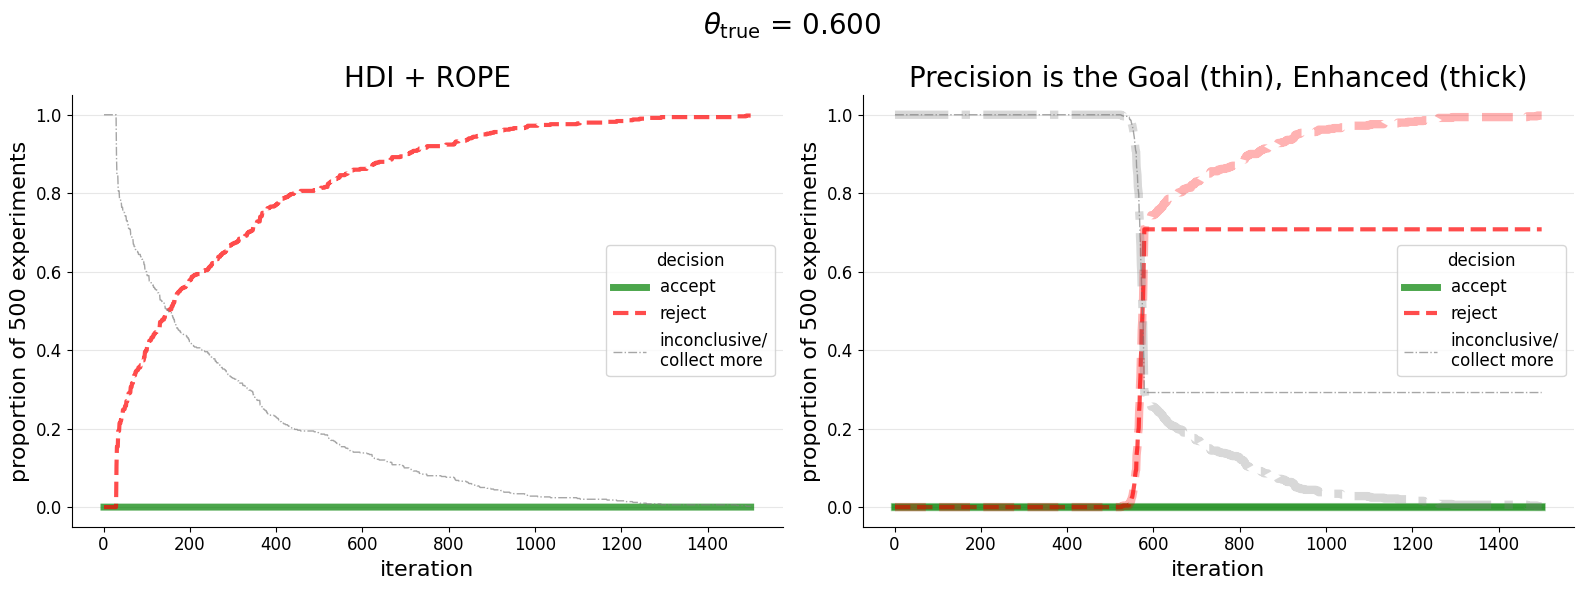
\includegraphics[width=1\textwidth]{loaded0pt6_experiment_decision_rates.png}
  \caption{Similar information as in Figure \ref{fig:fair_iter_vs_rate} but focusing on
  the distribution of decisions. Left panel is for HDI+ROPE. Right panel are both
  precision based methods. Horizontal axis- iteration. Vertical axis- proportion of
  decisions made up to (and including) each iteration. The sum of Reject (red dashed),
  Accept (green solid) and Inconclusive/Collect-more- (gray dot-dashed) decisions at
  each iteration is 100\%.
  }
  \label{fig:loaded0pt6_decisions}
\end{figure}